%!TEX root = ./template-skripsi.tex

\subsection{\textit{Sprint 6}}

	\textit{Sprint-6} dilakukan sepekan pada tanggal 27 September 2022 sampai dengan 4 oktober 2022. \textit{Story} keenam pada \textit{product backlog} yaitu membuat fitur treatment kolam dipecah menjadi beberapa \textit{task} sebagai berikut.


 \begin{longtable}[c]{@{} |p{1cm}|p{4cm}|p{5cm}|p{3cm}| @{}}
 \caption{\textit{Sprint 6} \label{sprint6_table}}\\


 \hline
  \multirow{1}{=}{\centering{\textbf{No}}} & \multirow{1}{=}{\centering{\textbf{\textit{Story}}}} & \multirow{1}{=}{\centering{\textbf{\textit{Task}}}} & \multirow{1}{=}{\centering{\textbf{\textit{Status}}}}\\
 \endfirsthead

 \hline
  \multirow{1}{=}{\centering{\textbf{No}}} & \multirow{1}{=}{\centering{\textbf{\textit{Story}}}} & \multirow{1}{=}{\centering{\textbf{\textit{Task}}}} & \multirow{1}{=}{\centering{\textbf{\textit{Status}}}}\\
 \endhead

 \hline
 \endfoot

 \hline
 \endlastfoot

 \hline
 1 & Membuat fitur treatment kolam &  Membuat \textit{Mock-up UI} halaman list treatment, detail treatment, entry treatment &  selesai \\
 \hline
 2 & & Menerapkan \textit{Mock-up UI} halaman list treatment, detail treatment, entry treatment  ke Flutter & selesai\\
 \hline
 \end{longtable}

Pada sprint keenam ini story yang di pilih untuk di uraikan pada sprint kali ini adalah membuat halaman rekapitulasi treatment, detail treatment, entry treatment. Tujuan dari \textit{sprint-6} ini adalah membuat fitur treatment berat ikan dan mengintegrasikan halaman tersebut dengan webservice yang sudah dibuat oleh penelitian Andri Rahmanto.
	


\begin{enumerate}[listparindent=2em]
	
	\item{\textit{Membuat Mock-up UI Fitur Treatment Kolam}}
	
	Pembuatan konten dan fitur yang terdapat pada \textit{mock-up UI} fitur treatment kolam dilakukan berdasarkan persetujuan product owner dan scrum master pada meeting sebelumnya. Mock-up UI dibuat menggunakan platform figma.
	
	\begin{figure}[H]
	\centering
	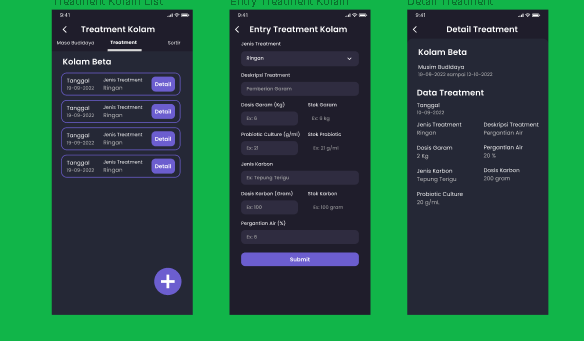
\includegraphics[keepaspectratio, width=6cm]{gambar/mockuptreatment}
	\caption{\textit{Mock-up UI Fitur treatment}}
	\label{gambar:mockuptreatment}
	\end{figure}

	\item{\textit{Class Diagram}}
	
	Class Diagram menggambarkan kelas-kelas yang akan dipakai oleh sistem. Umumnya terdapat 3 kelas pada setiap module yaitu class model, controller, dan view. Pada sprint-6 penelitian kali ini penulis membuat 4 class yaitu model yang berwarna biru, view berwarna oranye, controller yang berwarna hijau, dan service yang berwarna kuning.
	 
	 \begin{figure}[H]
	 \centering
	 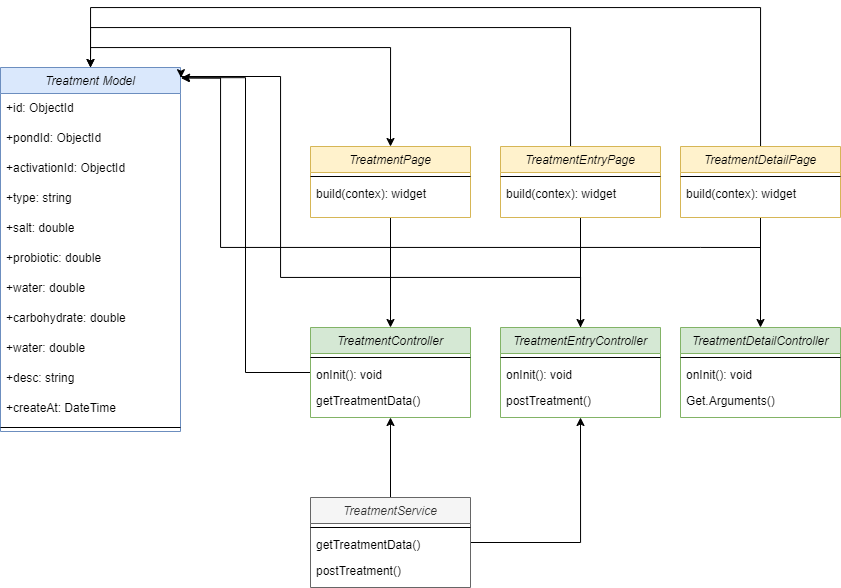
\includegraphics[keepaspectratio, width=6cm]{gambar/treatmentcd}
	 \caption{\textit{Class Diagram Fitur Sprint-6}}
	 \label{gambar:treatmentcd}
	 \end{figure}

	\item{\textit{Menerapkan Mockup-UI Fitur Treatment Kolam kedalam code flutter}}
	
	Setelah \textit{mock-up UI fitur treatment kolam}, akan dilakukan pengimplementasian \textit{mock-up UI} ke dalam aplikasi menggukan flutter. Pada lampiran 7 terdapat source code dari implementasi fitur treatment yang dikelompokan berdasarkan halaman yang menghasilkan halaman seperti dibawah ini.
	
	\begin{figure}[H]
		\centering
		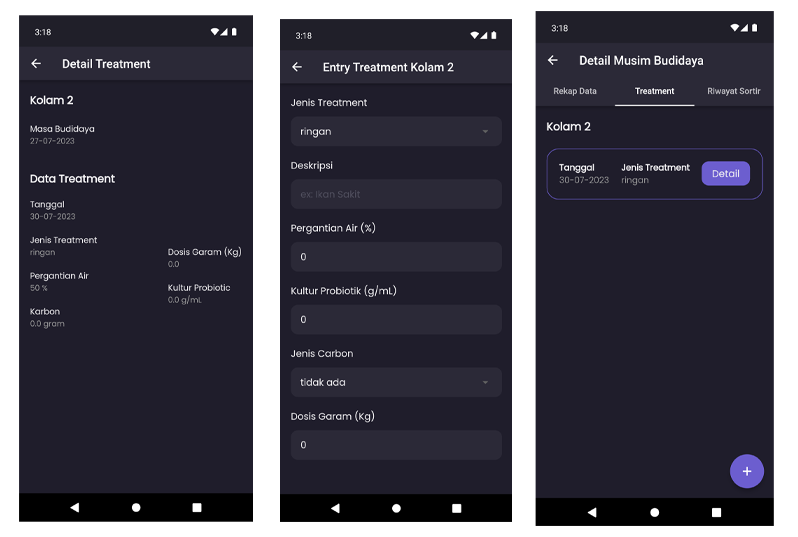
\includegraphics[keepaspectratio, width=8cm]{gambar/sssprint6}
		\caption{\textit{Output dari code pada sprint 6}}
		\label{gambar:sssprint6}
		\end{figure}

  \item{Analisis \textit{User Experience}} 
 
  Pada halaman entry treatment, pembudidaya harus memasukan data yang diperlukan untuk melakukan treatment kolam sesuai dengan kesepakatan saat meeting. Selain itu terdapat juga list mengenai data treatment yang telah dimasukan yang berisi informasi yang berhubungan dengan treatment kolam. Terdapat pula halaman detail treatment yang berisi informasi yang lebih detail terkait treatment yang telah dilakukan.

\item{Sprint 6 Review dan Sprint 7 Planning}

Sprint 6 diakhiri dengan melakukan weekly meeting pada hari selasa dengan agenda melakukan review dan testing terkait hasil sprint 6 dan melakukan planning untuk sprint 7 dengan rincian:
\begin{enumerate}
	\item{\textit{Review dan Testing hasil dari sprint 6}}

	Telah dilakukan review dan testing oleh penulis selaku developer dengan Scrum Master. Setelah dilakukan testing, Scrum Master menyimpulkan bahwa fitur treatment kolam telah berjalan dengan baik.

	\item{\textit{Sprint Planning untuk Sprint 7}}
	
	Planning untuk sprint 7 yakni membuat halaman untuk fitur treatment kolam pada aplikasi \textit{Assistive Aquaculture Breeding Management}.
\end{enumerate}
\end{enumerate}